%%
%% Automatically generated file from DocOnce source
%% (https://github.com/hplgit/doconce/)
%%
%%


%-------------------- begin preamble ----------------------

% Style: Lecture Notes in Computer Science (Springer)
\documentclass[a4paper]{llncs}

\listfiles               %  print all files needed to compile this document

\usepackage{relsize,epsfig,makeidx,color,setspace,amsmath,amsfonts,amssymb}
\usepackage[table]{xcolor}
\usepackage{bm,ltablex,microtype}

\usepackage{graphicx}

\usepackage[T1]{fontenc}
%\usepackage[latin1]{inputenc}
\usepackage{ucs}
\usepackage[utf8x]{inputenc}

\usepackage{lmodern}         % Latin Modern fonts derived from Computer Modern

% Hyperlinks in PDF:
\definecolor{linkcolor}{rgb}{0,0,0.4}
\usepackage{hyperref}
\hypersetup{
    breaklinks=true,
    colorlinks=true,
    linkcolor=linkcolor,
    urlcolor=linkcolor,
    citecolor=black,
    filecolor=black,
    %filecolor=blue,
    pdfmenubar=true,
    pdftoolbar=true,
    bookmarksdepth=3   % Uncomment (and tweak) for PDF bookmarks with more levels than the TOC
    }
%\hyperbaseurl{}   % hyperlinks are relative to this root

\setcounter{tocdepth}{2}  % levels in table of contents

% Tricks for having figures close to where they are defined:
% 1. define less restrictive rules for where to put figures
\setcounter{topnumber}{2}
\setcounter{bottomnumber}{2}
\setcounter{totalnumber}{4}
\renewcommand{\topfraction}{0.95}
\renewcommand{\bottomfraction}{0.95}
\renewcommand{\textfraction}{0}
\renewcommand{\floatpagefraction}{0.75}
% floatpagefraction must always be less than topfraction!
% 2. ensure all figures are flushed before next section
\usepackage[section]{placeins}
% 3. enable begin{figure}[H] (often leads to ugly pagebreaks)
%\usepackage{float}\restylefloat{figure}

% prevent orhpans and widows
\clubpenalty = 10000
\widowpenalty = 10000

% --- end of standard preamble for documents ---


%\usepackage{amsthm}
%\theoremstyle{definition}
%\newtheorem{remark}{Remark}
%\newtheorem{example}{Example}
%\newtheorem{definition}{Definition}


\usepackage{algorithm, algpseudocode}
\renewcommand{\algorithmicrequire}{\textbf{Input:}}
\renewcommand{\algorithmicensure}{\textbf{Output:}}

\pagestyle{plain}
\thispagestyle{plain}

% insert custom LaTeX commands...

\raggedbottom
\makeindex
\usepackage[totoc]{idxlayout}   % for index in the toc
\usepackage[nottoc]{tocbibind}  % for references/bibliography in the toc

%-------------------- end preamble ----------------------

\begin{document}

% matching end for #ifdef PREAMBLE

% \newcommand{\exercisesection}[1]{\subsection*{#1}}

\newcommand{\msize}[1]{{\left|#1\right|}}
\newcommand{\Nei}[2]{N_{#1}(#2)}
\newcommand{\Neiclosed}[2]{N_{#1}[#2]}
\newcommand{\bfI}{I}
\newcommand{\bfJ}{J}
\newcommand{\onestep}{\leftrightarrow}
\newcommand{\sevstep}{\leftrightsquigarrow}
\newcommand{\sevstepT}[1]{\overset{#1}{\leftrightsquigarrow}}
\newcommand{\calS}{{\cal S}}
\newcommand{\calSp}{{\calS^\prime}}
\newcommand{\calSpp}{{\calS^{\prime\prime}}}
\newcommand{\calP}{{\cal P}}
\newcommand{\sfTS}{{\sf TS}}
\newcommand{\sfTJ}{{\sf TJ}}
\newcommand{\sfTAR}{{\sf TAR}}
\newcommand{\sfPSPACE}{\sf PSPACE}
\newcommand{\RigidSet}[1]{{\mathsf R}({#1})}
\newcommand{\ConfinedCliques}[1]{{\mathsf K}{(#1)}}
\newcommand{\bfIstar}{\bfI^*}
\newcommand{\bfIp}{\bfI^{\prime}}
\newcommand{\bfIpp}{\bfI^{\prime\prime}}
\newcommand{\bfJp}{\bfJ^{\prime}}
\newcommand{\bfJpp}{\bfJ^{\prime\prime}}
\newcommand{\Gp}{{G^\prime}}
\newcommand{\Gpp}{G^{\prime\prime}}
\newcommand{\Gstar}{G^*}
\newcommand{\Bp}{B^{\prime}}
\newcommand{\Bpp}{B^{\prime\prime}}
\newcommand{\Bstar}{B^*}
\newcommand{\dist}{\mathsf{dist}}


% ------------------- main content ----------------------



% ----------------- title -------------------------

\mainmatter
\title{Sliding Tokens on Block Graphs}
% Short version of title:
\titlerunning{Sliding Tokens on Block Graphs}

% ----------------- author(s) -------------------------

\author{Duc A. Hoang\inst{1}
\and
Eli Fox-Epstein\inst{2}
\and
Ryuhei Uehara\inst{1}}
\institute{JAIST, Japan
\email{\{hoanganhduc, uehara\}@jaist.ac.jp}
\and
Brown University, USA
\email{ef@cs.brown.edu}}
% ----------------- end author(s) -------------------------

\maketitle

\abstract{
Let $I, J$ be two given independent sets of a graph $G$.
Imagine that the vertices of an independent set are viewed as tokens (coins).
A token is allowed to move (or slide) from one vertex to one of its neighbors.
The {\sc Sliding Token} problem asks whether there exists a sequence of independent sets of $G$ starting from $I$ and ending with $J$ such that each intermediate member of the sequence is obtained from the previous one by moving a token according to the allowed rule.
In this paper, we claim that this problem is solvable in polynomial time when the input graph is a block graph---a graph whose blocks are cliques.
Our algorithm is developed based on the characterization of a non-trivial structure that, in certain conditions, can be used to indicate a {\sc no}-instance of the problem.
Without such a structure, a sequence of token slidings between any two independent sets of the same cardinality exists.
}

\section{Introduction}
\label{sec:introduction}

Recently, motivated by the purpose of understanding the solution space of a problem, many theoretical computer scientists have focused on the study of \emph{reconfiguration problems}.
\emph{Reconfiguration problems} are the set of problems in which we are given a collection of
\emph{feasible solutions}, together with some \emph{reconfiguration rule(s)} that defines an \emph{adjacency relation} on the set of feasible solutions of the original problem. 
The question is, using a reconfiguration rule, whether there is a step-by-step transformation which transforms one feasible solution to another, such that each intermediate result is also feasible.
A simple example is the famous Rubik's cube puzzle.
The reconfigurability of several well-known problems, including 
	{\sc satisfiability},
	{\sc independent set},
	{\sc vertex-colouring}, 
	{\sc matching},
	{\sc clique}, etc.
	have been studied extensively.
For more information about this research area, see the survey \cite{Heuvel2013}.

As the {\sc independent set} problem is one of the most important problems in the computational complexity theory, its reconfiguration variants have been well-studied \cite{HearnDemaine2005,IDHPSUU,KaminskiMedvedevMilanic2012}.
Recall that an \emph{independent set} of a graph is a set of pairwise non-adjacent vertices.
Among these variants, the {\sc Sliding Token} problem (first introduced by Hearn and Demaine \cite{HearnDemaine2005}) is of particular interest (see \cite{KaminskiMedvedevMilanic2012} for the other variants).
Given two independent sets $\bfI$ and $\bfJ$ of a graph $G$, 
	and imagine that a token is placed on each vertex in $\bfI$. 
Then, the {\sc Sliding Token} problem asks
whether there exists a sequence (called a $\sfTS$-\emph{sequence}) 
$\calS = \langle \bfI_1, \bfI_2, \ldots, \bfI_{\ell} \rangle$ of independent sets of $G$ such that

\begin{itemize}
\item [(a)] $\bfI_1=\bfI$, $\bfI_{\ell}=\bfJ$, and $\msize{\bfI_i} = \msize{\bfI}=\msize{\bfJ}$ for all $i$, $1 \le i \le \ell$; and 

\item [(b)] for each $i$, $1 \le i \le \ell-1$, there is an edge $uv$ in $G$ such that $\bfI_{i} \setminus\bfI_{i+1}=\{u\}$ and $\bfI_{i+1}\setminus\bfI_{i}=\{v\}$.
\end{itemize}

\noindent
If such a sequence $\calS$ exists, we say that $\calS$ \emph{reconfigures} $\bfI$ to $\bfJ$ in $G$ and write $\bfI \sevstepT{G} \bfJ$. 
An example of a $\sfTS$-sequence is given in \figurename~\ref{fig:exa-TS-seq}. 
Observe that `` $\sevstepT{G}$ '' is indeed an equivalence relation.
{\sc Sliding Token} is $\sfPSPACE$-complete even for planar graphs \cite{HearnDemaine2005} and bounded-treewidth graphs \cite{MouawadNishimuraRamanWrochna}.
On the positive side, polynomial-time algorithms have been designed recently for claw-free graphs \cite{BonsmaKaminskiWrochna}, cographs \cite{KaminskiMedvedevMilanic2012}, trees \cite{DDFEHIOOUY2015}, bipartite permutation graphs \cite{FoxEpsteinHoangOtachiUehara2015}, and cactus graphs \cite{Hoang2016cactus}.

% original latex figure with scale=1


\begin{figure}[!ht]  % fig:exa-TS-seq
  \centerline{\includegraphics[scale=1.0]{fig/exa-TS-seq.eps}}
  \caption{
  Example of a $\sfTS$-sequence $\langle \bfI_1, \bfI_2, \dots, \bfI_5 \rangle$ in a given graph that reconfigures $\bfI_1$ to $\bfI_5$. The vertices in independent sets are depicted by black circles (tokens). \label{fig:exa-TS-seq}
  }
\end{figure}
%\clearpage % flush figures fig:exa-TS-seq


A \emph{block} of a graph $G$ is a maximal connected subgraph with no cut vertex.
A \emph{block graph} is a graph whose blocks are cliques (for example, see the graph in \figurename~\ref{fig:exa-TS-seq}).
Note that, in order to preserve the independence property of the set of tokens, a token sometimes needs to make ``detours''.
This restriction indeed makes {\sc Sliding Token} more complicated (recall that the problem is $\sfPSPACE$-complete even for bounded-treewidth graphs), even when the input graph is a tree (see \cite{DDFEHIOOUY2015}).
As there might be exponential number of paths between any two vertices of a block graph (while in a tree, there is a unique path), 
	for each token, we may have exponentially many choices of ``routes'' to slide and possibly super polynomial detours in general.
Thus, in this case, the problem becomes more difficult.
In this paper, we design a polynomial-time algorithm for solving the {\sc Sliding Token} problem for block graphs. 

Our algorithm is designed based on the following observations.
Given a block graph $G$ and an independent set $\bfI$ of $G$, 
	one can characterize the properties of a non-trivial structure, called $(G, \bfI)$-\emph{confined clique} (Section~\ref{sec:confined-cliques}).
More precisely, we claim that one can find all $(G, \bfI)$-confined cliques in polynomial time (Lemma~\ref{lem:check-confined-in-polytime}), 	
	and, in certain conditions, we can easily derive if an instance of {\sc Sliding Token} is a {\sc no}-instance (Lemma~\ref{lem:no-instance}).
Without such a structure, we claim that for any pair of independent sets $\bfI, \bfJ$, $\bfI$ is reconfigurable to $\bfJ$ (and vice versa) if and only if they are of the same cardinality (Lemma~\ref{lem:yes-instance-if-same-size}).

Due to the limitation of space, some proofs are omitted.

\section{Preliminaries}
\label{sec:preliminaries}

\subsection*{Graph notation}
\label{sec:graph-notation}

We define some notation that is commonly used in graph theory.
For the notation that is not mentioned here, see \cite{Diestel2010}.
Let $G$ be a given graph, with edge set $E(G)$ and vertex set $V(G)$.

We sometimes denote by $\msize{G}$ the size of $V(G)$.
For a vertex $v$, we define $\Nei{G}{v} = \{w \in V(G): vw \in E(G)\}$, $\Neiclosed{G}{v} = \Nei{G}{v} \cup \{v\}$ and $\deg_G(v) = |\Nei{G}{v}|$. 
For two vertices $u, v$, we denote by $\dist_G(u, v)$ the \emph{distance} between $u$ and $v$ in $G$.
For a graph $G$, sometimes we write $\bfI \cap G$ and $\bfI - G$ to indicate the sets $\bfI \cap V(G)$ and $\bfI \setminus V(G)$, respectively.

For $X \subseteq V(G)$, we denote by $G[X]$ the subgraph of $G$ \emph{induced} by vertices of $X$.
We write $G - X$ to indicate the graph $G[V(G) \setminus X]$.
Similarly, for an induced subgraph $H$ of $G$, $G - H$ indicates the graph $G[V(G) \setminus V(H)]$, 
	and we say that the graph $G - H$ is obtained by \emph{removing $H$ from $G$}.

\subsection*{Notation for {\sc Sliding Token}}
\label{sec:TS-notation}

We now define some useful notation for tackling {\sc Sliding Token}. 
For a $\sfTS$-sequence $\calS$, we write $\bfI \in \calS$ if an independent set $\bfI$ of $G$ appears in $\calS$. 
For a vertex $v$, if there exists $\bfI \in \calS$ such that $v \in \bfI$, then we say that $\calS$ \emph{involves} $v$.
We say that $\calS = \langle \bfI_1, \bfI_2, \ldots, \bfI_{\ell} \rangle$  \emph{slides} (or \emph{moves}) the token $t$ placed at $u \in \bfI_1$ to $v \notin \bfI_1$ in $G$ if after applying the sliding steps described in $\calS$, the token $t$ is placed at $v \in \bfI_\ell$.
For convenience, we sometimes identify the token placed at a vertex with the vertex itself, and simply say ``a token in an independent set $\bfI$.''

Let $W \subseteq V(G)$ and assume that $\bfI \cap W \neq \emptyset$. 
We say that a token $t$ placed at some vertex $u \in \bfI \cap W$ is $(G, \bfI, W)$-\emph{confined} 
	if for every $\bfJ$ such that $\bfI \sevstepT{G} \bfJ$, 
	$t$ is always placed at some vertex of $W$.
In other words, $t$ can only be slid along edges of $G[W]$.
In case $W = \{u\}$, $t$ is said to be $(G, \bfI)$-\emph{rigid}.
The token $t$ is $(G, \bfI)$-\emph{movable} if it is not $(G, \bfI)$-rigid.

Let $H$ be an induced subgraph of $G$.
$H$ is called $(G, \bfI)$-\emph{confined} if
	$\bfI \cap H$ is a maximum independent set of $H$
	and all tokens in $\bfI \cap H$ are $(G, \bfI, V(H))$-confined.
In particular, if $H$ is a clique of $G$, we say that it is a $(G, \bfI)$-\emph{confined clique}.
Note that if $H$ is a clique then $\msize{\bfI \cap H} \leq 1$.
We denote by $\ConfinedCliques{G, \bfI}$ the set of all $(G, \bfI)$-confined cliques of $G$.
For a vertex $v \in V(H)$, we define $G^v_H$ 
	to be the (connected) component of $G_H$ containing $v$, where $G_H$ is obtained from $G$ by removing all edges of $H$.

\section{Some useful observations}
\label{sec:useful-observations}

In this section, we present several useful observations.
These observations will be implicitly used in many statements of this paper.
The next proposition characterizes some properties of a $(G, \bfI)$-confined induced subgraph.


\begin{proposition}[{\cite[Lemma 1]{Hoang2016cactus}}]
\label{prop:extra-properies}
Let $\bfI$ be an independent set of a graph $G$.
Let $H$ be an induced subgraph of $G$.
Then the following conditions are equivalent.

\begin{itemize}
\item [(i)] $H$ is $(G, \bfI)$-confined.

\item [(ii)] For every independent set $\bfJ$ satisfying $\bfI \sevstepT{G} \bfJ$, $\bfJ \cap H$ is a maximum independent set of $H$.

\item [(iii)] $\bfI \cap H$ is a maximum independent set of $H$ and for every $\bfJ$ satisfying $\bfI \sevstepT{G} \bfJ$, any token $t_x$ placed at $x \in \bfJ \cap H$ is $(G^x_H, \bfJ \cap G^x_H)$-rigid.
\end{itemize}

\noindent
\end{proposition}


The next proposition says that when $G$ is disconnected, one can deal with each component separately. In other words, when dealing with {\sc Sliding Token}, it suffices to consider only connected graphs.


\begin{proposition}[{\cite[Proposition 2]{Hoang2016cactus}}]
\label{prop:TS-in-each-compoenent}
Let $\bfI$, $\bfJ$ be two given independent set of $G$.
Assume that $G_1, \dots, G_k$ are the components of $G$. 
Then $\bfI \sevstepT{G} \bfJ$ if and only if $\bfI \cap G_i \sevstepT{G_i} \bfJ \cap G_i$ for $i = 1, 2, \dots, k$.
\end{proposition}


In the next proposition, we claim that in certain conditions, a $\sfTS$-sequence in a subgraph of $G$ can be somehow ``extended'' to a sequence in $G$, and vice versa.


\begin{proposition}[{\cite[Proposition 3]{Hoang2016cactus}}]
\label{prop:TS-in-subgraphs}
Let $u$ be a vertex of a graph $G$.
Let $\calS = \langle \bfI_1, \bfI_2, \dots, \bfI_\ell \rangle$ be a $\sfTS$-sequence in $G$ such that for any $\bfI \in \calS$, $u \in \bfI$.
Let $\Gpp = G - \Neiclosed{G}{u}$.
Then $\bfI_1 \cap \Gp \sevstepT{\Gpp} \bfI_\ell \cap \Gp$.
Moreover, for any $\sfTS$-sequence $\calSp = \langle \bfIp_1, \dots, \bfIp_l \rangle$ in $\Gpp$, $\bfIp_1 \cup \{u\} \sevstepT{G} \bfIp_l \cup \{u\}$.
\end{proposition}


In case $G$ is a block graph, we also have:


\begin{proposition}
\label{prop:TS-in-subgraphs-blockgraph}
Let $\bfI$ be an independent set of a block graph $G$.
Let $B$ be a block of $G$ and suppose that $\bfI \cap B = \{u\}$.
Let $\calS = \langle \bfI_1, \bfI_2, \dots, \bfI_\ell \rangle$ be a $\sfTS$-sequence in $G$ such that for any $\bfJ \in \calS$, $u \in \bfJ$.
Let $\Gp = G - B$.
Then $\bfI_1 \cap \Gp \sevstepT{\Gp} \bfI_\ell \cap \Gp$.
Moreover, for any $\sfTS$-sequence $\calSp = \langle \bfIp_1, \dots, \bfIp_l \rangle$ in $\Gp$ such that $\Nei{G}{u} \cap \bfIp_i = \emptyset$, where $i \in \{1, 2, \dots, \ell\}$, $\bfIp_1 \cup \{u\} \sevstepT{G} \bfIp_l \cup \{u\}$.
\end{proposition}



\begin{proposition}
\label{prop:every-token-is-not-confined}
Let $G$ be a block graph and let $\bfI$ be an independent set of $G$.
Let $v \in V(G)$ be such that no token in $\Nei{G}{v} \cap \bfI$ is $(G, \bfI, \Neiclosed{G}{v})$-confined.
Then there exists an independent set $\bfJ$ of $G$ such that $\bfI \sevstepT{G} \bfJ$ and $\Neiclosed{G}{v} \cap \bfJ = \emptyset$.
\end{proposition}



\begin{proposition}
\label{prop:confined-token-in-closed-neghbor}
Let $\bfI$ be an independent set of a block graph $G$.
Let $w \in V(G)$. 
Assume that no block of $G$ containing $w$ is $(G, \bfI)$-confined. 
If there exists some vertex $x \in \Neiclosed{G}{w} \cap \bfI$ such that the token $t_x$ placed at $x$ is $(G, \bfI, \Neiclosed{G}{w})$-confined, 
	then $x$ is unique.
Consequently, there must be some independent set $\bfJ$ such that $\bfI \sevstepT{G} \bfJ$ and $\Neiclosed{G}{w} \cap \bfJ = \{x\}$.
Moreover, let $H$ be the graph obtained from $G$ by turning $\Neiclosed{G}{w}$ into a clique, called $B_w$.
Then $t_x$ is $(G, \bfJ, \Neiclosed{G}{w})$-confined if and only if $B_w$ is $(H, \bfJ)$-confined.
\end{proposition}


\section{Confined cliques in block graphs}
\label{sec:confined-cliques}

In this section, we show that one can compute $\ConfinedCliques{G, \bfI}$ in polynomial time, where $G$ is a block graph and $\bfI$ is an independent set of $G$.
First, we prove an useful characterization of $(G, \bfI)$-confined cliques.


\begin{lemma}
\label{lem:characterize-confined-clique}
Let $\bfI$ be an independent set of a block graph $G$.
Let $B$ be a block of $G$ with $\bfI \cap B \neq \emptyset$.
Let $\Gp = G - B$.
Then $B$ is $(G, \bfI)$-confined (see \figurename~\ref{fig:characterize-confined-cliques}(a)) if and only if either $G = B$ or for every cut vertex $v \in V(B)$, one of the following conditions holds.

\begin{itemize}
\item [(i)] There exists a block $\Bp \neq B$ of $G$ containing $v$ such that $\Bp - v$ is $(\Gp, \bfI \cap \Gp)$-confined (for example, the vertices $v_1$ and $v_2$ in \figurename~\ref{fig:characterize-confined-cliques}(a)).

\item [(ii)] For every block $\Bp \neq B$ of $G$ containing $v$, $\Bp - v$ is not $(\Gp, \bfI \cap \Gp)$-confined; and for every $w \in \Nei{G}{v} \setminus V(B)$, either
\begin{itemize}

  \item [(ii-1)] there exists a block $\Bpp$ of $\Gp$ containing $w$ such that $\Bpp$ is $(\Gp, \bfI \cap \Gp)$-confined (for example, the vertex $v_4$ in \figurename~\ref{fig:characterize-confined-cliques}(a)); or

  \item [(ii-2)] every block $\Bpp$ of $\Gp$ containing $w$ is not $(\Gp, \bfI \cap \Gp)$-confined;  and there exists $x \in \Neiclosed{\Gp}{w} \cap \bfI$ such that the token $t_x$ placed at $x$ is $(\Gp, \bfI \cap \Gp, \Neiclosed{\Gp}{w})$-confined (for example, the vertex $v_3$ in \figurename~\ref{fig:characterize-confined-cliques}(a)).
\end{itemize}

\noindent
\end{itemize}

\noindent
\end{lemma}


% original latex figure with scale=0.6


\begin{figure}[!ht]  % fig:characterize-confined-cliques
  \centerline{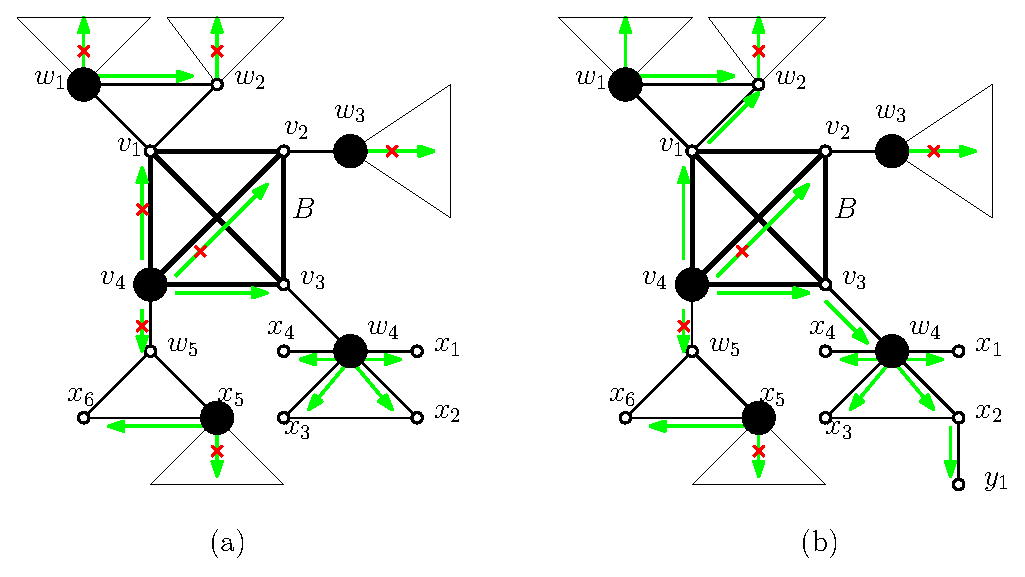
\includegraphics[scale=0.6]{fig/characterize-confined-cliques.eps}}
  \caption{
  (a) $B$ is $(G, \bfI)$-confined and (b) $B$ is not $(G, \bfI)$-confined. \label{fig:characterize-confined-cliques}
  }
\end{figure}
%\clearpage % flush figures fig:characterize-confined-cliques


Next, we characterize $(G, \bfI)$-rigid tokens.


\begin{lemma}
\label{lem:characterize-rigid-token}
Let $\bfI$ be an independent set of a block graph $G$.
Let $u \in \bfI$.
The token $t$ placed at $u$ is $(G, \bfI)$-rigid (see \figurename~\ref{fig:characterize-rigid-tokens}) if and only if 
	for every $v \in \Nei{G}{u}$, 
	there exists a vertex $w \in \big(\Nei{G}{v} \setminus \{u\}\big) \cap \bfI$ such that one of the following conditions holds.

\begin{itemize}
\item [(i)] The token $t_w$ placed at $w$ is $(\Gpp, \bfI \cap \Gpp)$-rigid, where $\Gpp = G - \Neiclosed{G}{u}$ (for example, the vertex $w_1$ in \figurename~\ref{fig:characterize-rigid-tokens}(a)).

\item [(ii)] The token $t_w$ placed at $w$ is not $(\Gpp, \bfI \cap \Gpp)$-rigid; and the block $\Bp$ of $G$ containing $v$ and $w$ satisfies that $\Bp - v$ is $(\Gpp, \bfI \cap \Gpp)$-confined (for example, the vertices $w_3$ and $w_4$ in \figurename~\ref{fig:characterize-rigid-tokens}(a)).
\end{itemize}

\noindent
\end{lemma}


% original latex figure with scale=0.6


\begin{figure}[!ht]  % fig:characterize-rigid-tokens
  \centerline{\includegraphics[scale=0.6]{fig/characterize-rigid-tokens.eps}}
  \caption{
  (a) The token placed at $u$ is $(G, \bfI)$-rigid and (b) The token placed at $u$ is $(G, \bfI)$-movable. \label{fig:characterize-rigid-tokens}
  }
\end{figure}
%\clearpage % flush figures fig:characterize-rigid-tokens


The next lemma says that one can compute all $(G, \bfI)$-confined blocks in polynomial time, where $G$ is a block graph and $\bfI$ is an independent set of $G$.


\begin{lemma}
\label{lem:check-confined-in-polytime}
Let $\bfI$ be an independent set of a block graph $G$.
Let $m = \msize{E(G)}$.
Let $B$ be a block of $G$ with $\bfI \cap B \neq \emptyset$.
Then, one can check if $B$ is $(G, \bfI)$-confined in $O(m)$ time.
Consequently, one can compute $\ConfinedCliques{G, \bfI}$ in $O(m^2)$ time.
\end{lemma}



\begin{proof}

We describe a recursive function {\sc CheckConfined}($G$, $\bfI$, $H$) which returns {\sc yes} if an input induced subgraph $H$ is $(G, \bfI)$-confined, where $\bfI$ is an independent set of $G$ and $H$ is either a clique or a vertex.
Otherwise, it returns {\sc no} and a $\sfTS$-sequence $\calS_H$ in $G$ which slides the token in $\bfI \cap H$ (if exists) to a vertex in $\bigcup_{v \in V(H)}\Nei{G}{v} \setminus V(H)$.
Clearly, if $\bfI \cap H = \emptyset$ then {\sc CheckConfined}($G$, $\bfI$, $H$) returns {\sc no} and there is no such $\calS_H$ described above.
Thus, we now assume that $\bfI \cap H \neq \emptyset$.
Note that since $H$ is either a clique or a vertex, $\msize{\bfI \cap H} = 1$.
By definition, it is clear that if $G = H$ then {\sc CheckConfined}($G$, $\bfI$, $H$) returns {\sc yes}.
Then, we now consider the case when $G \neq H$, i.e., $G$ contains more than one block.
Let $u$ be the unique vertex in $\bfI \cap H$, and $t_u$ be the token placed at $u$.
Let $\Gp = G - H$ and $\Gpp = G - \Neiclosed{G}{u}$.
If $H$ is a clique, we will use Lemma~\ref{lem:characterize-confined-clique} to check if $H$ is $(G, \bfI)$-confined.
On the other hand, if $H$ contains only vertex $u$ (i.e., $H = (\{u\}, \emptyset)$), we will use Lemma~\ref{lem:characterize-rigid-token} to check if $H$ is $(G, \bfI)$-confined (by definition, it is equivalent to checking if $t_u$ is $(G, \bfI)$-rigid).

If $H$ is a clique, then by Lemma~\ref{lem:characterize-confined-clique}, 
	for every cut vertex $v \in V(H)$,
	we need to check if one of the conditions (i), (ii) of Lemma~\ref{lem:characterize-confined-clique} holds.
Note that since $v$ is a cut vertex, there is at least one block $\Bp \neq H$ of $G$ containing $v$.
To check if Lemma~\ref{lem:characterize-confined-clique}(i) holds, we recursively call {\sc CheckConfined}($\Gp$, $\bfI \cap \Gp$, $\Bp - v$) for every block $\Bp \neq H$ of $G$ containing $v$.
If {\sc CheckConfined}($\Gp$, $\bfI \cap \Gp$, $\Bp - v$) returns {\sc no} for all blocks $\Bp \neq H$ of $G$ containing $v$, i.e.~Lemma refaux{lem:characterize-confined-clique}(i) does not hold, 
	we can construct a $\sfTS$-sequence $\calS_v$ in $G$ that slides $t_u$ to $v$ as follows.
If $u = v$ then nothing needs to be done.
Thus, we assume that $u \neq v$, which then implies that $v \notin \bfI$.
In order to slide $t_u$ to $v$, we need to make sure that for every block $\Bp \neq H$ of $G$ containing $v$, if $\bfI \cap (\Bp - v) \neq \emptyset$, 
	the token in $\bfI \cap (\Bp - v)$ need to be moved to a vertex not in $\Bp - v$ first.
To do this, note that for each such $\Bp$, the function {\sc CheckConfined}($\Gp$, $\bfI \cap \Gp$, $\Bp - v$) also returns a $\sfTS$-sequence $\calS_{\Bp - v}$ in $\Gp$ that slides the token in $\bfI \cap (\Bp - v)$ to a vertex in $\bigcup_{x \in V(\Bp - v)}\Nei{\Gp}{x} \setminus V(\Bp - v)$.
By Proposition~\ref{prop:TS-in-subgraphs-blockgraph}, such a sequence $\calS_{\Bp - v}$ can indeed be performed in $G$.
Hence, $\calS_v$ can be constructed (using the results from {\sc CheckConfined}($\Gp$, $\bfI \cap \Gp$, $\Bp - v$)) by first performing all $\calS_{\Bp - v}$, then performing a single step of sliding $t_u$ to $v$.  
If Lemma~\ref{lem:characterize-confined-clique}(i) does not hold, for every $w \in \Nei{G}{v} \setminus V(H)$, we need to check if Lemma~\ref{lem:characterize-confined-clique}(ii) holds.
We first need to check whether there exists a block $\Bpp$ of $\Gp$ containing $w$
	such that $\Bpp$ is $(\Gp, \bfI \cap \Gp)$-confined.
This can be done by calling {\sc CheckConfined}($\Gp$, $\bfI \cap \Gp$, $\Bpp$) for all blocks $\Bpp$ of $\Gp$ containing $w$ such that $\bfI \cap \Bpp \neq \emptyset$.
If the result is {\sc no} for every such $\Bpp$, i.e., Lemma~\ref{lem:characterize-confined-clique}(ii-1) does not hold, 
	we still need to check if  Lemma~\ref{lem:characterize-confined-clique}(ii-2) holds.
To do this, we consider the following cases.

\begin{itemize}
\item [$\circ$] \textbf{Case 1:} $\msize{\Neiclosed{\Gp}{w} \cap \bfI} = 0$.
\end{itemize}

\noindent
In this case, Lemma~\ref{lem:characterize-confined-clique}(iii) does not hold, which then implies that {\sc CheckConfined}($G$, $\bfI$, $H$) returns {\sc no}.
To see this, we shall construct a $\sfTS$-sequence $\calS_H$ in $G$ that slides $t_u$ to $w \in \Nei{G}{v} \setminus V(H)$.
Indeed, $\calS_H$ can be constructed by simply performing two steps of sliding: $t_u$ to $v$, and then $t_u$ from $v$ to $w$ (since $\msize{\Neiclosed{\Gp}{w} \cap \bfI} = 0$). 
\begin{itemize}
\item [$\circ$] \textbf{Case 2:} $\msize{\Neiclosed{\Gp}{w} \cap \bfI}  = 1$.
\end{itemize}

\noindent
Let $K$ be the block graph obtained from $\Gp$ by turning $\Neiclosed{\Gp}{w}$ into a clique, called $B_w$.
By Proposition~\ref{prop:confined-token-in-closed-neghbor}, checking if Lemma~\ref{lem:characterize-confined-clique}(iii) holds is equivalent to checking if $B_w$ is $(K, \bfI)$-confined.
In case Lemma~\ref{lem:characterize-confined-clique}(iii) holds, 
	the construction of $\calS_H$ can be done by 
	first sliding the token in $\Neiclosed{\Gp}{w} \cap \bfI$ to some vertex not in $\Neiclosed{\Gp}{w} \cap \bfI$ (converting a $\sfTS$-sequence in $K$ to a $\sfTS$-sequence in $\Gp$ as in Proposition~\ref{prop:confined-token-in-closed-neghbor}, 
	and extending that $\sfTS$-sequence to a $\sfTS$-sequence in $G$ using Proposition~\ref{prop:TS-in-subgraphs-blockgraph}), 
	and then use the process described in \textbf{Case 1} to slide $t_u$ to $w$. 
\begin{itemize}
\item [$\circ$] \textbf{Case 3:} $\msize{\Neiclosed{\Gp}{w} \cap \bfI} \geq 2$.
\end{itemize}

\noindent
We first show how to construct an independent set $\bfJ$ such that $\bfI \sevstepT{G} \bfJ$ and $\msize{\Neiclosed{\Gp}{w} \cap \bfJ} \leq 1$.
Note that since $\msize{\Neiclosed{\Gp}{w} \cap \bfI} \geq 2$, we have $w \notin \bfI$.
The idea of this construction comes from Proposition~\ref{prop:every-token-is-not-confined} and Proposition~\ref{prop:confined-token-in-closed-neghbor}.
Proposition~\ref{prop:confined-token-in-closed-neghbor} indeed implies that there is at most one token $t_x$ in $\Neiclosed{\Gp}{w} \cap \bfI$ that is $(\Gp, \bfI \cap \Gp, \Neiclosed{\Gp}{w})$-confined.
In other words, all tokens in $\Neiclosed{\Gp}{w} \cap \bfI$ except $t_x$ (if exists) can be slid to a vertex not in $\Neiclosed{\Gp}{w}$.
Now, for each block $\Bpp$ of $\Gp$ containing $w$ with $\bfI \cap \Bpp \neq \emptyset$, from the results of calling {\sc CheckConfined}($\Gp$, $\bfI \cap \Gpp$, $\Bpp$), 
	we obtain a $\sfTS$-sequence $\calS_{\Bpp}$ in $\Gp$ (which can also be extended in $G$ using Proposition~\ref{prop:TS-in-subgraphs-blockgraph}) that moves the token in $\bfI \cap \Bpp$ to a vertex not in $\Bpp$.
Note that $\calS_{\Bpp}$ may or may not contain the step of sliding the token in $\bfI \cap \Bpp$ to $w$.
If for some block $\Bpp$ of $\Gp$ containing $w$ with $\bfI \cap \Bpp \neq \emptyset$, $\calS_{\Bpp}$ contains such a step, then clearly it will move all other tokens in $\bfI \cap \Neiclosed{\Gp}{w}$ ``out of'' $\Neiclosed{\Gp}{w}$ first,
	and then moves the token in $\bfI \cap \Bpp$ to $w$.
Stop at this point, we obtain an independent set $\bfJ$ such that $\bfI \sevstepT{G} \bfJ$ and $\msize{\Neiclosed{\Gp}{w} \cap \bfJ} = 1$.
The only token in $\Neiclosed{\Gp}{w} \cap \bfJ$ is now indeed the token placed at $w$. 
On the other hand, if for all blocks $\Bpp$ of $\Gp$ containing $w$ with $\bfI \cap \Bpp \neq \emptyset$, $\calS_{\Bpp}$ does not contain the step of sliding the token in $\bfI \cap \Bpp$ to $w$,
	then we simply perform all such $\calS_{\Bpp}$.
Since $G$ is a block graph, all such $\calS_{\Bpp}$ can indeed be performed independently, 
	i.e., no sequence involves any vertex that is involved by other sequences.
At the end of this process, we obtain an independent set $\bfJ$ such that $\bfI \sevstepT{G} \bfJ$ and $\msize{\Neiclosed{\Gp}{w} \cap \bfJ} = 0$.
Once we have $\bfJ$, the checking process can indeed be done using either \textbf{Case 1} or \textbf{Case 2}. 
Keep in mind that the construction of $\bfJ$ uses only the results that can be obtained from the recursive callings of the {\sc CheckConfined} function.

In the above arguments, we have analyzed the cases that {\sc CheckConfined}($G$, $\bfI$, $H$) returns {\sc no} using Lemma~\ref{lem:characterize-confined-clique}, where $H$ is a clique.
In all other cases, {\sc CheckConfined}($G$, $\bfI$, $H$) indeed returns {\sc yes} (by Lemma~\ref{lem:characterize-confined-clique}).

If $H$ contains only a single vertex $u$, then by Lemma~\ref{lem:characterize-rigid-token}, we need to check that for every $v \in \Nei{G}{u}$, 
	whether there exists a vertex $w \in \big(\Nei{G}{v} \setminus \{u\}\big) \cap \bfI$ such that 
	one of the conditions (i), (ii) of Lemma~\ref{lem:characterize-rigid-token} holds.
Clearly, if $\big( \Nei{G}{v} \setminus \{u\} \big) \cap \bfI = \emptyset$, one can construct a $\sfTS$-sequence $\calS_H$ that slides $t_u$ to $v$ by performing the single step of sliding $t_u$ to $v$, and hence {\sc CheckConfined}($G$, $\bfI$, $H$) returns {\sc no}.
Next, we consider the case when  $\big( \Nei{G}{v} \setminus \{u\} \big) \cap \bfI \neq \emptyset$.
In this case, for every $w \in  \big( \Nei{G}{v} \setminus \{u\} \big) \cap \bfI$, we recursively call {\sc CheckConfined}($\Gpp$, $\bfI \cap \Gpp$, $\{w\}$) to check if Lemma~\ref{lem:characterize-rigid-token}(i) holds.
If {\sc CheckConfined}($\Gpp$, $\bfI \cap \Gpp$, $\{w\}$) = {\sc no} for all $w \in \big( \Nei{G}{v} \setminus \{u\} \big) \cap \bfI$, we still need to check if Lemma~\ref{lem:characterize-rigid-token}(ii) holds by calling {\sc CheckConfined}($\Gpp$, $\bfI \cap \Gpp$, $B_w - v$) for all $w \in \big( \Nei{G}{v} \setminus \{u\} \big) \cap \bfI$, where $B_w$ denotes the (unique) block of $G$ containing both $v, w$.
If {\sc CheckConfined}($\Gpp$, $\bfI \cap \Gpp$, $B_w - v$) returns {\sc no} for all $w \in \big( \Nei{G}{v} \setminus \{u\} \big) \cap \bfI$, we can indeed return {\sc no} for the function {\sc CheckConfined}($G$, $\bfI$, $H$).
The $\sfTS$-sequence $\calS_H$ that moves $t_u$ to $v$ in this case can be constructed as follows.
For each $w \in \big( \Nei{G}{v} \setminus \{u\} \big) \cap \bfI$, since {\sc CheckConfined}($\Gpp$, $\bfI \cap \Gpp$, $B_w - v$) returns {\sc no}, there must be a $\sfTS$-sequence $\calS_{\Bp - v}$ in $\Gpp$ (which can be extended to $G$ using Proposition~\ref{prop:TS-in-subgraphs}) that slides the token in $\bfI \cap (\Bp - v)$ to a vertex in $\bigcup_{z \in V(\Bp - v)}\Nei{\Gp}{\Bp - v} \setminus V(\Bp - v)$.
$\calS_H$ then can be constructed by first performing all such $\calS_{\Bp - v}$, and then performing a single step of sliding $t_u$ to $v$.
In the above arguments, we have analyzed the cases that {\sc CheckConfined}($G$, $\bfI$, $H$) returns {\sc no} using Lemma~\ref{lem:characterize-rigid-token}, where $H$ is a vertex.
In all other cases, {\sc CheckConfined}($G$, $\bfI$, $H$) indeed returns {\sc yes} (by Lemma~\ref{lem:characterize-rigid-token}).

Next, we analyze the complexity of the described algorithm.
First of all, note that all the $\sfTS$-sequences mentioned in the described algorithm can indeed be construction using the results from the recursive callings of the {\sc CheckConfined} function.
Thus, the running time of our algorithm is indeed proportional to the number of callings of the {\sc CheckConfined} function.
For a vertex $v \in V(G)$, let $f(v)$ be the number of calling {\sc CheckConfined} \emph{related} to $v$, in the sense that the function {\sc CheckConfined} is either called for $v$ or for a block containing $v$.
Thus, the total number of callings {\sc CheckConfined} is indeed bounded by $\sum_{v \in V(G)}f(v)$.
Moreover, from the described algorithm, note that $f(v)$ is at most $O(\deg_G(v))$.
Hence, checking if $H$ is $(G, \bfI)$-confined takes at most $O(\sum_{v \in V(G)}\deg_G(v)) = O(m)$ time, where $H$ is either a clique or a vertex.
Consequently, since the number of blocks of $G$ is $O(m)$, computing $\ConfinedCliques{G, \bfI}$ takes at most $O(m^2)$ time.

\end{proof}


\section{Sliding tokens on block graphs}
\label{sec:TS-on-block-graphs}

Let $G$ be a block graph, and let $\bfI, \bfJ$ be two independent sets of $G$.
In this section, we prove the following main result of this paper.


\begin{theorem}
\label{thrm:main}
Let $(G, \bfI, \bfJ)$ be an instance of the {\sc Sliding Token} problem, where $\bfI, \bfJ$ are two independent sets of a block graph $G$.
Then, one can decide if $\bfI \sevstepT{G} \bfJ$ in $O(m^2)$ time, where $m = \msize{E(G)}$.
\end{theorem}


To prove Theorem~\ref{thrm:main}, we shall describe a polynomial-time algorithm for deciding if $\bfI \sevstepT{G} \bfJ$, estimate its running time, and then prove its correctness.
The following algorithm checks if $\bfI \sevstepT{G} \bfJ$.

\begin{itemize}
\item [$\circ$] \textbf{Step 1:}
\begin{itemize}

  \item [$\bullet$] \textbf{Step 1-1:} If $\ConfinedCliques{G, \bfI} \neq \ConfinedCliques{G, \bfJ}$, return {\sc no}.

  \item [$\bullet$] \textbf{Step 1-2:} Otherwise, remove all cliques in $\ConfinedCliques{G, \bfI}$ and go to \textbf{Step 2}. Let $\Gp$ be the resulting graph.

\end{itemize}

\noindent
\item [$\circ$] \textbf{Step 2:} If $\msize{\bfI \cap F} \neq \msize{\bfJ \cap F}$ for some component $F$ of $\Gp$, return {\sc no}. Otherwise, return {\sc yes}.
\end{itemize}

\noindent
We now analyze the time complexity of the algorithm.
Let $m, n$ be respectively the number of edges and vertices of $G$.
By Lemma~\ref{lem:check-confined-in-polytime}, \textbf{Step 1-1} takes at most $O(m^2)$ time.
\textbf{Step 1-2} clearly takes at most $O(n)$ time.
Hence, \textbf{Step 1} takes at most $O(m^2)$ time.
\textbf{Step 2} takes at most $O(n)$ time.
In total, the algorithm runs in $O(m^2)$ time.

The rest of this section is devoted to showing the correctness of the algorithm.
First of all, the following lemma is useful.

\begin{lemma}
\label{lem:one-block}
Let $\bfI$ be an independent set of a block graph $G$.
Let $w \in V(G)$. 
Assume that every block of $G$ containing $w$ is not $(G, \bfI)$-confined. 
Then, there is at most one block $B$ of $G$ containing $w$ such that $B - w$ is $(\Gp, \bfI \cap \Gp)$-confined, where $\Gp = G - w$.
\end{lemma}


The next lemma ensures the correctness of \textbf{Step 1-1}.


\begin{lemma}
\label{lem:no-instance}
Let $(G, \bfI, \bfJ)$ be an instance of the {\sc Sliding Token} problem, where $\bfI, \bfJ$ are two independent sets of a block graph $G$.
Then, it is a {\sc no}-instance if $\ConfinedCliques{G, \bfI} \neq \ConfinedCliques{G, \bfJ}$.
\end{lemma}


In the next lemma, we claim that \textbf{Step 1-2} is correct.


\begin{lemma}
\label{lem:remove-all-confined-cliques}
Let $(G, \bfI, \bfJ)$ be an instance of the {\sc Sliding Token} problem, where $\bfI, \bfJ$ are two independent sets of a block graph $G$ satisfying that $\ConfinedCliques{G, \bfI} = \ConfinedCliques{G, \bfJ}$.
Let $\Gp$ be the graph obtained from $G$ by removing all cliques in $\ConfinedCliques{G, \bfI} = \ConfinedCliques{G, \bfJ}$.
Then, $\bfI \sevstepT{G} \bfJ$ if and only if $\bfI \cap \Gp \sevstepT{\Gp} \bfJ \cap \Gp$.
Furthermore, $\ConfinedCliques{\Gp, \bfI \cap \Gp} = \ConfinedCliques{\Gp, \bfJ \cap \Gp} = \emptyset$.
\end{lemma}



\begin{proof}

Let $\calS = \langle \bfI = \bfI_1, \bfI_2, \dots, \bfI_\ell = \bfJ \rangle$ be a $\sfTS$-sequence in $G$ that reconfigures $\bfI$ to $\bfJ$.
We claim that there exists a $\sfTS$-sequence $\calSp$ in $\Gp$ that reconfigures $\bfI \cap \Gp$ to $\bfJ \cap \Gp$.
Note that for any independent set $\bfI$ of $G$, $\bfI \cap \Gp$ forms an independent set of $\Gp$.
Moreover, for $i = 1, 2, \dots, \ell - 1$, let $uv$ be an edge of $G$ such that $u \in \bfI_i \setminus \bfI_{i+1}$ and $v \in \bfI_{i+1} \setminus \bfI_i$, then clearly $u$ and $v$ must be either both in $\Gp$ or both in some block $B \in \ConfinedCliques{G, \bfI}$.
Hence, the sequence $\calSp = \langle \bfI_1 \cap \Gp, \dots, \bfI_\ell \cap \Gp \rangle$ reconfigures $\bfI_1 \cap \Gp = \bfI \cap \Gp$ to $\bfI_\ell \cap \Gp = \bfJ \cap \Gp$.

Let $\calSp = \langle \bfI \cap \Gp = \bfIp_1, \bfIp_2, \dots, \bfIp_l = \bfJ \cap \Gp \rangle$ be a $\sfTS$-sequence in $\Gp$ that reconfigures $\bfI \cap \Gp$ to $\bfJ \cap \Gp$.
We claim that there exists a $\sfTS$-sequence $\calS$ in $G$ that reconfigures $\bfI = (\bfI \cap \Gp) \cup \bigcup_{B \in \ConfinedCliques{G, \bfI}}(\bfI \cap B)$ to $\bfJ = (\bfJ \cap \Gp) \cup \bigcup_{B \in \ConfinedCliques{G, \bfI}}(\bfJ \cap B)$.
Note that for an independent set $\bfIp$ of $\Gp$ and a block $B \in \ConfinedCliques{G, \bfI}$, it is not necessary that $\bfIp \cup (\bfIpp \cap B)$ forms an independent set of $G$,
	where $\bfIpp$ is an independent set of $G$ such that $\bfI \sevstepT{G} \bfIpp$.
For a component $F$ of $\Gp$, one can construct a $\sfTS$-sequence $\calSp_F = \langle \bfIp_1 \cap F, \dots, \bfIp_l \cap F \rangle$ in $F$. 
We now describe how to construct $\calS$.
Let $A = \bigcup_{B \in \ConfinedCliques{G, \bfI}}\bigcup_{v \in \bfI \cap B}\big( \Nei{G}{v} \cap V(F) \big)$.
For a component $F$ of $\Gp$, we consider the following cases.

\begin{itemize}
\item [$\circ$] $\calSp_F$ \textbf{does not involve any vertex in} $A$.
\end{itemize}

\noindent
In this case, note that for every independent set $\bfI_F$ of $F$ and a block $B \in \ConfinedCliques{G, \bfI}$, the set $\bfI_F \cup (\bfJ \cap B)$ forms an independent set of $G$, where $\bfJ$ is any independent set of $G$ satisfying $\bfI \sevstepT{G} \bfJ$.
Thus, such a sequence $\calSp_F$ above indeed can be ``extended'' to a $\sfTS$-sequence in $G$.
\begin{itemize}
\item [$\circ$] $\calSp_F$ \textbf{involves vertices in} $A$.
\end{itemize}

\noindent
Note that for a block $B \in \ConfinedCliques{G, \bfI}$, 
	since $G$ is a block graph, 
	there is at most one vertex $v \in V(B)$ satisfying that $\Nei{G}{v} \cap V(F) \neq \emptyset$.
Moreover, if there exists two vertices $u_1, u_2 \in V(F)$ such that $\Nei{G}{u_i} \cap V(B) \neq \emptyset$ ($i = 1, 2$) then they must be adjacent to the same vertex in $B$.
Let $v$ be the unique vertex in $\bfI \cap B$ and assume that $\Nei{G}{v} \cap V(F) \neq \emptyset$.
Then, the token $t_v$ placed at $v$ must not be $(G, \bfI)$-rigid.
To see this, note that, if the token $t$ placed at $u \in \bfI$ is $(G, \bfI)$-rigid, then by definition of confined cliques, any block of $G$ containing $u$ must be in $\ConfinedCliques{G, \bfI}$. 
Hence, for a block $B \in \ConfinedCliques{G, \bfI}$ and $v \in \bfI \cap B$ with $\Nei{G}{v} \cap V(F) \neq \emptyset$, there exists a $\sfTS$-sequence $\calSp(B, v)$ in $G$ that moves the token $t_v$ placed at $v$ to some other vertex in $B$.
Since $G$ is a block graph, if there are two of such block $B$, say $B_1$ and $B_2$, with $v_1 \in \bfI \cap B_1$ and $v_2 \in \bfI \cap B_2$,
	then clearly $\calSp(B_1, v_1)$ does not involve any token which is involved by $\calSp(B_2, v_2)$ (and vice versa). 

Now, we construct a $\sfTS$-sequence $\calS$ in $G$ that reconfigures $\bfI$ to $\bfJ$ as follows.
First, we perform all $\sfTS$-sequence $\calSp_F$ that does not involve any vertex in $A$.
Next, for a component $F$ with the corresponding sequence $\calSpp_F$ involving  
	let $B \in \ConfinedCliques{G, \bfI}$ such that there exists a (unique) vertex $v \in \bfI \cap B$ satisfying that $\Nei{G}{v} \cap V(F) \subseteq A$.
For such component $F$ and such block $B$, we first perform $\calSp(B, v)$, then perform $\calSp_F$, and then perform $\calSp(B, v)$ in reverse order.
Note that if after performing $\calSp(B, v)$, the token $t_v$ (originally placed at $v$) is placed at some vertex $w \in \bfJ$, then in the step of reversing $\calSp(B, v)$, we do not reverse the step of sliding $t_v$ to $w$.
At this moment, we have reconfigured $\bfI \cap \Gp$ to $\bfJ \cap \Gp$ in $G$. 
It remains to reconfigure $\bfI \cap B$ to $\bfJ \cap B$ in $G$ for each block $B \in \ConfinedCliques{G, \bfI}$, which can be done using the observation that for any vertex $v \in \bfJ \cap B$, $\Nei{G}{v} \cap \bfJ \neq \emptyset$.

Finally, we claim that $\ConfinedCliques{\Gp, \bfI \cap \Gp} = \emptyset$.
Similar arguments can also be applied for showing $\ConfinedCliques{\Gp, \bfJ \cap \Gp} = \emptyset$.
Assume for the contradiction that there exists some block $B^\prime \in \ConfinedCliques{\Gp, \bfI \cap \Gp}$.
Let $v$ be the unique vertex in $\bfI \cap B^\prime$, and let $B$ be the block of $G$ containing $\Bp$.
We consider the following cases.

\begin{itemize}
\item [$\circ$] $B = \Bp$.
\end{itemize}

\noindent
Note that since $\Bp$ is a block of both $G$ and $\Gp$, 
	it follows that $\Bp$ is not $(G, \bfI)$-confined.
In other words, there exists a $\sfTS$-sequence $\calS$ in $G$ that slides the token $t_v$ placed at $v \in \bfI \cap \Bp$ to some vertex not in $\Bp$.
Moreover, as before, we have proved that such a $\sfTS$-sequence can indeed be ``restricted'' to $\Gp$ based on the observation that 
	for any independent set $\bfI$ of $G$, $\bfI \cap \Gp$ forms an independent set of $\Gp$ 
	and any sliding step is performed either along edges of $\Gp$ or along edges of some $(G, \bfI)$-confined block.
Therefore, $\Bp$ is not $(\Gp, \bfI \cap \Gp)$-confined, a contradiction.
\begin{itemize}
\item [$\circ$] $\msize{V(B) \setminus V(B^\prime)} = 1$.
\end{itemize}

\noindent
Let $w$ be the unique vertex in $V(B) \setminus V(B^\prime)$. 
Note that since $w$ is a vertex of some $(G, \bfI)$-confined block $C \neq B$, the token $t_v$ placed at $v$ cannot be slid to $w$ in $G$.
Since $B$ is not $(G, \bfI)$-confined, as before, there exists a $\sfTS$-sequence $\calS$ in $G$ that slides the token $t_v$ placed at $v \in \bfI \cap \Bp$ to some vertex not in $\Bp$.
Moreover, $\calS$ does not move $t_v$ to $w$, which means that it moves $t_v$ to some vertex of $\Gp$ that is not in $\Bp$.
Thus, $\calS$ can indeed be ``restricted'' to $\Gp$, which means that $\Bp$ is indeed not $(\Gp, \bfI \cap \Gp)$-confined, a contradiction.

\end{proof}


Before proving the correctness of \textbf{Step 2}, we need some extra definitions.
Let $B$ be a block of a block graph $G$.
A block $\Bp \neq B$ of $G$ is called a \emph{neighbor} of $B$ if $V(B) \cap V(\Bp) \neq \emptyset$.
$B$ is called \emph{safe} if it has at most one cut vertex and at most one neighbor having more than one cut vertex.
A vertex $v \in V(G)$ is called \emph{safe} if it is a non-cut vertex of a safe block of $G$.

The next two lemmas are useful for showing the correctness of \textbf{Step 2}.


\begin{lemma}
\label{lem:slide-tokens-to-safe-vertex}
Let $\bfI$ be an independent set of a block graph $G$ such that $\ConfinedCliques{G, \bfI} = \emptyset$.
Let $v$ be a safe vertex of $G$.
Then, there exists an independent set $\bfJ$ of $G$ with $\bfI \sevstepT{G} \bfJ$ and $v \in \bfJ$.
\end{lemma}



\begin{lemma}
\label{lem:remove-safe-block}
Let $\bfI$ be an independent set of a block graph $G$ such that $\ConfinedCliques{G, \bfI} = \emptyset$.
Let $v \in \bfI$ be a safe vertex of $G$ and let $B_v$ be the (unique) safe block of $G$ containing $v$.
Let $\Gstar$ be the subgraph of $G$ obtained by removing $B_v$.
Then, $\ConfinedCliques{\Gstar, \bfI \cap \Gstar} = \emptyset$.
\end{lemma}


The following lemma ensures the correctness of \textbf{Step 2}.


\begin{lemma}
\label{lem:yes-instance-if-same-size}

Let $(G, \bfI, \bfJ)$ be an instance of the {\sc Sliding Token} problem, where $\bfI, \bfJ$ are two independent sets of a block graph $G$ satisfying that $\ConfinedCliques{G, \bfI} = \ConfinedCliques{G, \bfJ} = \emptyset$.
Then, $\bfI \sevstepT{G} \bfJ$ if and only if $\msize{\bfI} = \msize{\bfJ}$.
\end{lemma}



\begin{proof}

The only-if-part is trivial.
We shall prove the if-part, i.e., if $\msize{\bfI} = \msize{\bfJ}$ then $\bfI \sevstepT{G} \bfJ$.
More precisely, we claim that there exists an independent set $\bfIstar$ such that $\bfI \sevstepT{G} \bfIstar$ and $\bfJ \sevstepT{G} \bfIstar$.
Indeed, $\bfIstar$ can be constructed as follows.
Initially, $\bfIstar = \emptyset$.

\begin{itemize}
\item [$\circ$] Pick a safe vertex $v$ of $G$. (Note that the ``tree-like'' structure of a block graph ensures that one can always find a safe block, and hence a safe vertex.)

\item [$\circ$] Slide a token from $\bfI$ and a token from $\bfJ$ to $v$.
\end{itemize}

\noindent
Then, add $v$ to $\bfIstar$.
This can be done using Lemma~\ref{lem:slide-tokens-to-safe-vertex}.
Let $\bfIp$ and $\bfJp$ be the resulting independent sets.
\begin{itemize}
\item [$\circ$] Let $\Gp$ be the graph obtained by removing $B_v$ - the (unique) block of $G$ containing $v$.

\item [$\circ$] Repeat the above steps with the new triple $(\Gp, \bfIp \setminus \{v\}, \bfJp \setminus \{v\})$ instead of $(G, \bfI, \bfJ)$. The procedure stops when there is no token to move.
\end{itemize}

\noindent
The correctness of this construction is followed from Lemma~\ref{lem:slide-tokens-to-safe-vertex} and Lemma~\ref{lem:remove-safe-block}.

\end{proof}


\subsubsection*{Acknowledgement.}

The first author would like to thank Yota Otachi for his useful discussions. 
This work is partially supported by MEXT/JSPS Kakenhi Grant Number 26330009 and 24106004.



\bibliographystyle{splncs}
\bibliography{references}



% ------------------- end of main content ---------------

\end{document}

